\documentclass[tikz,border=8pt]{standalone}
\usepackage{tikz}
\usetikzlibrary{arrows.meta,positioning,shapes.geometric}
\begin{document}
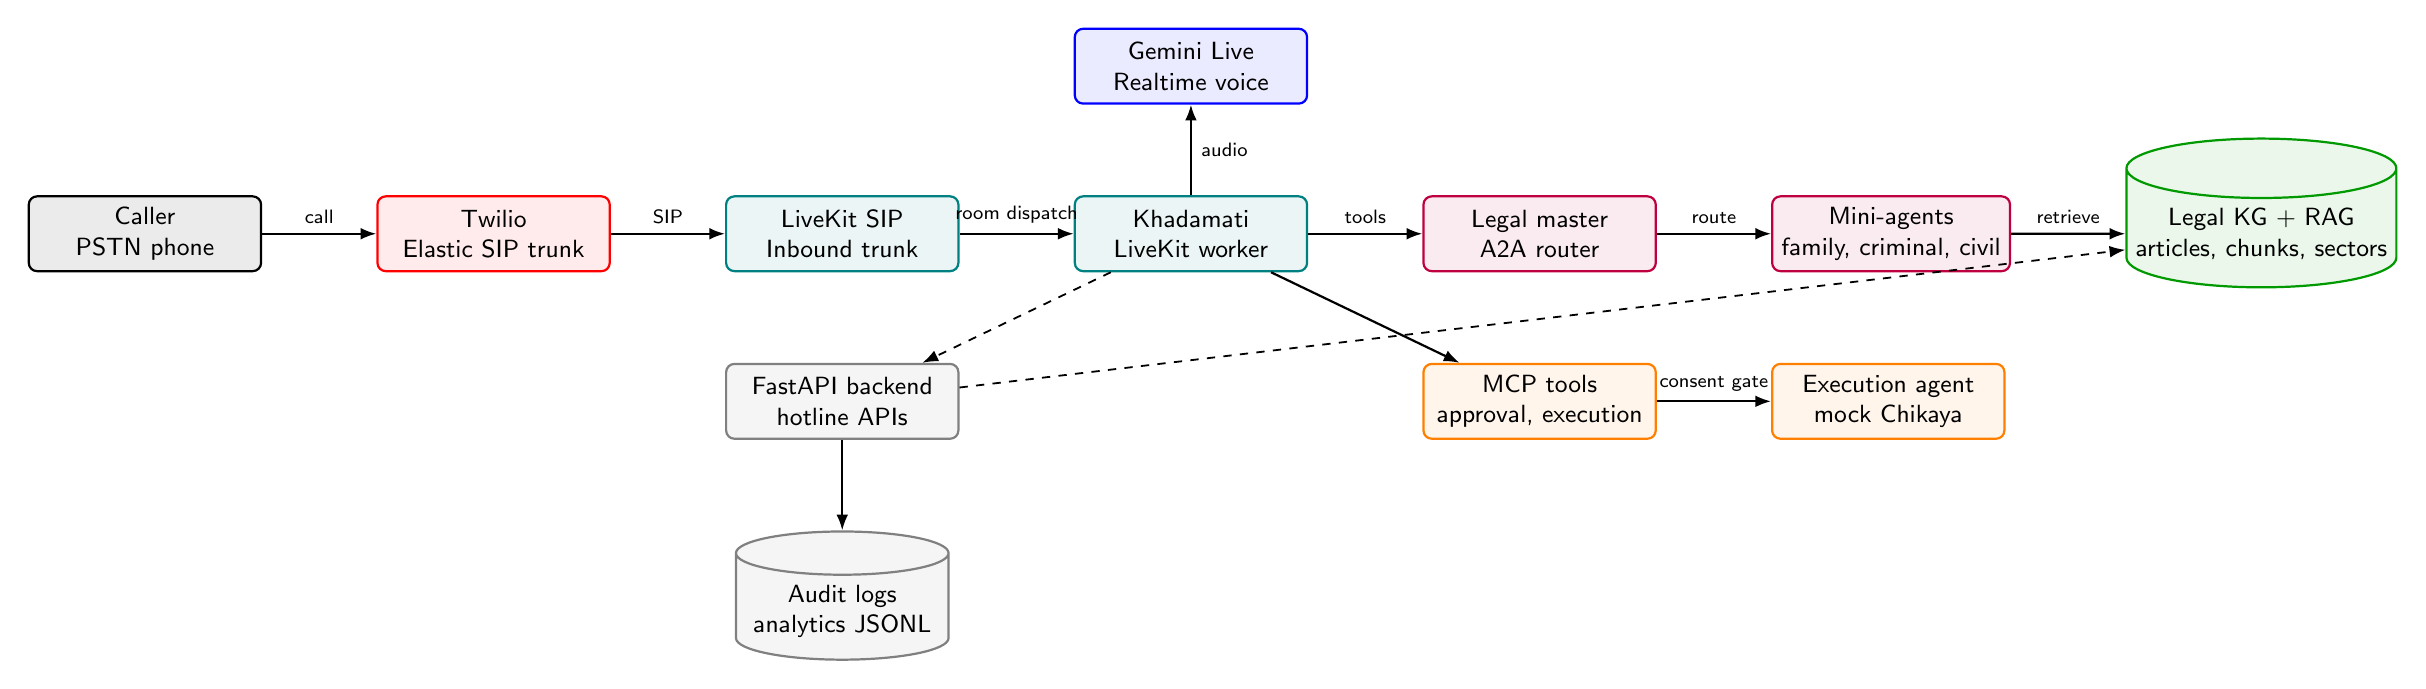
\begin{tikzpicture}[
  node distance=1.15cm and 1.45cm,
  box/.style={draw=#1, fill=#1!8, rounded corners=3pt, line width=0.8pt, align=center, minimum width=2.95cm, minimum height=0.95cm, font=\sffamily\small},
  store/.style={draw=#1, fill=#1!8, cylinder, shape border rotate=90, aspect=0.22, line width=0.8pt, align=center, minimum width=2.7cm, minimum height=1.05cm, font=\sffamily\small},
  arrow/.style={-{Latex[length=2mm]}, line width=0.8pt},
  muted/.style={-{Latex[length=2mm]}, dashed, line width=0.65pt}
]
  \node[box=black] (caller) {Caller\\PSTN phone};
  \node[box=red, right=of caller] (twilio) {Twilio\\Elastic SIP trunk};
  \node[box=teal, right=of twilio] (sip) {LiveKit SIP\\Inbound trunk};
  \node[box=teal, right=of sip] (agent) {Khadamati\\LiveKit worker};
  \node[box=blue, above=of agent] (gemini) {Gemini Live\\Realtime voice};
  \node[box=purple, right=of agent] (master) {Legal master\\A2A router};
  \node[box=purple, right=of master] (experts) {Mini-agents\\family, criminal, civil};
  \node[store=green!60!black, right=of experts] (kg) {Legal KG + RAG\\articles, chunks, sectors};
  \node[box=orange, below=of master] (mcp) {MCP tools\\approval, execution};
  \node[box=orange, right=of mcp] (exec) {Execution agent\\mock Chikaya};
  \node[box=gray, below=of sip] (backend) {FastAPI backend\\hotline APIs};
  \node[store=gray, below=of backend] (logs) {Audit logs\\analytics JSONL};

  \draw[arrow] (caller) -- node[above, font=\sffamily\scriptsize]{call} (twilio);
  \draw[arrow] (twilio) -- node[above, font=\sffamily\scriptsize]{SIP} (sip);
  \draw[arrow] (sip) -- node[above, font=\sffamily\scriptsize]{room dispatch} (agent);
  \draw[arrow] (agent) -- node[right, font=\sffamily\scriptsize]{audio} (gemini);
  \draw[arrow] (agent) -- node[above, font=\sffamily\scriptsize]{tools} (master);
  \draw[arrow] (master) -- node[above, font=\sffamily\scriptsize]{route} (experts);
  \draw[arrow] (experts) -- node[above, font=\sffamily\scriptsize]{retrieve} (kg);
  \draw[arrow] (agent) -- (mcp);
  \draw[arrow] (mcp) -- node[above, font=\sffamily\scriptsize]{consent gate} (exec);
  \draw[arrow] (backend) -- (logs);
  \draw[muted] (agent) -- (backend);
  \draw[muted] (backend) -- (kg);
\end{tikzpicture}
\end{document}
